\documentclass[conference]{IEEEtran}

\IEEEoverridecommandlockouts

\usepackage[utf8]{inputenc}
\usepackage[T1]{fontenc}
\usepackage{cite}

\ifCLASSINFOpdf
  \usepackage[pdftex]{graphicx}
\else

\fi

\usepackage[cmex10]{amsmath}

\usepackage{multirow}
\usepackage{array}
\usepackage[lofdepth,lotdepth]{subfig}
\usepackage{color}
\usepackage{tabto}

\usepackage{amssymb}
\usepackage{booktabs}
\usepackage{multirow}
\usepackage{rotating}
\usepackage{amsmath}
\usepackage{algorithm}
\usepackage{algpseudocode}
\usepackage{lineno,hyperref}
\usepackage{graphicx}
\usepackage{pdflscape}
\usepackage[none]{hyphenat}

\begin{document}

\IEEEpubid{\makebox[\columnwidth]{\hfill} \hspace{\columnsep}\makebox[\columnwidth]{}}

\title{Makine Öğrenmesi Algoritmaları ile İkinci El Araç Fiyat Tahmini
\\
\*

Used Car Price Prediction with Machine Learning Algorithms
}
\author{
	
\IEEEauthorblockN{Samed ZIRHLIOĞLU}
\IEEEauthorblockA{Bilgisayar Mühendisliği\\
	18110131037\\
	Kahramanmaraş Sütçü İmam Üniversitesi\\
	Kahramanmaraş, Türkiye\\
	zirhlioglusamed@gmail.com
	}
\and
\IEEEauthorblockN{Mehtap ÖKLÜ}
\IEEEauthorblockA{Bilgisayar Mühendisliği\\
	17110131052\\
	Kahramanmaraş Sütçü İmam Üniversitesi\\
	Kahramanmaraş, Türkiye\\
	mehtap\_oklu\_06@hotmail.com
	}
}
\maketitle
\thispagestyle{plain}
\pagestyle{plain}
\begin{ozet}
Araçlar hayatımızda çok eskiden beri var olan ve hayatımızı kolaylaştıran icatlardır. Özellikle günümüzde, artık hayatımızın her alanında olmazsa olmazlarımızdandır. Bu göz önüne alınarak bir çok marka ve model üretilmiştir. Bu markalardan birisi de BMW’ dir. BMW’ nin her yıla özel ve farklı özelliklerde birçok modeli mevcuttur. Bu araçların özellikleri (model, yıl, şanzıman, mil, yakıt tipi, vergi, mesafe başına yakıt tüketimi, motor, fiyat) incelenerek aracın değeri tahmin edilebilir. Bu değerleri incelemek için yapay zeka algoritmalarını (Karar Ağacı, Gradient Boost, XGB, Rastgele Orman Ağacı, LightGBM, CatBoost) kullandık. Kullandığımız algoritmaların tamamı regresyon algoritmalarından oluşmakta. Bunun nedeni ise elimizdeki bağımsız değişkenlerden hareketle, yeni bir bağımlı değişken elde etmek istememizdir.
\end{ozet}

\begin{IEEEanahtar}
Araç, Araç Özellikleri, Karar Ağacı, Gradient Boost, XGB, Rastgele Orman Ağacı, LightGBM, CatBoost
\end{IEEEanahtar}

\begin{abstract}
Vehicles are inventions that have existed in our lives for a long time and make our lives easier. Especially nowadays, it is now an indispensable part of our lives. With this in mind, many brands and models have been produced. One of these brands is BMW. BMW has many models with different features and specific to each year. The value of the vehicle can be estimated by examining the characteristics of these vehicles (model, year, transmission, miles, fuel type, tax, fuel consumption per distance, engine, price). We used artificial intelligence algorithms (Decision Tree, Gradient Boost, XGB, Random Forest Tree, LightGBM, CatBoost) to examine these values. All of the algorithms we use are regression algorithms. The reason for this is that we want to obtain a new dependent variable based on the independent variables we have.
\end{abstract}

\begin{IEEEkeywords}
Car, Car Properties, Value, Decision Tree, Gradient Boost, XGB, Random Forest Tree, LightGBM, CatBoost
\end{IEEEkeywords}

\section{\textbf{GİRİŞ}}
\quad Ulaşım, insanlık tarihinin başlangıcından günümüze kadar, insan hayatının en temel ihtiyaçlarından birisi olmuştur. Arabalar icat edilmeden önce ulaşım; at, eşek ve deve gibi hayvanlar kullanılarak sağlanmıştı. Bu durum hem zaman hem de emek kaybına neden olmuştur.

\quad Artan dünya nüfusu ve ihtiyaçlar doğrultusunda ulaşım çok büyük bir önem kazanmıştır. Bu ihtiyaçları gidermek ve ulaşımı daha kolay hale getirmek için yapılan çalışmalar hız kazanmıştır. Bu çalışmalar sonucunda insanlar ihtiyaçları doğrultusunda tarım ve ulaşım araçlarını geliştirmiştir. İlerleyen süreçte ise insanların daha konforlu ve keyifli bir ulaşım deneyimi yaşayabilmesi için çalışmalara devam edilmiştir.

\quad Günümüzde otomobil sektörü, insanlık tarihinin en yaygın sektörlerinden ve yatırım yapılan iş kollarından  birisi olmuştur. Başlangıçta sadece ulaşım ve ticaret amaçlı kullanılan otomobiller, günümüzde lüks ve ihtişamlı yaşamın sembolü haline gelmiştir\cite{1}.

\quad Arabalar uzun ömürlü oldukları için sürekli alınıp satılabilir. İkinci el olarak satılan araçların makul bir şekilde fiyatlandırılması gerekir. İkinci el bir aracın makul fiyat tahmininin yapılması zordur. Bu nedenle, ikinci el araçlar için doğru fiyat tahmin mekanizmasına ihtiyaç vardır\cite{2}. Bu makalede yapay zeka kullanarak ikinci el araçların fiyatlarını tahmin etmeye çalışacağız.

\quad Bu proje için, "100.000 UK Used Car Dataset" isimli veri setini\cite{3} Kaggle’dan temin ettik. Elde ettiğimiz veri seti içerisinden BMW marka aracın verilerini alarak gerekli ön işleme adımlarını yaptık. Veri setimizde 8 adet öznitelik (model, yıl, şanzıman, satış fiyatı, mil, yıllık vergisi, mesafe başına yakıt miktarı ve motor hacmi) bulunmaktadır. Düzenlediğimiz verilerin \%30'unu test, \%70'ini eğitim verisi olarak ayırdık.

Kullandığımız özniteliklerin özellikleri;
\begin{itemize}
\item \textbf{Model:} Markanın sınıflara ayırdığı farklı araç tiplerine verdiği isim
\item \textbf{Yıl:} Aracın üretilip satışa sunulduğu yıl
\item \textbf{Şanzıman:} Motordan istenilen hareketi şaft veya diferansiyele aktarma organıdır.
\item \textbf{Satış fiyatı:} Aracın son durumundaki satış fiyatı
\item \textbf{Mil:} Aracın gittiği toplam yol
\item \textbf{Yıllık vergi:} Devletin araç kullananlardan düzenli olarak aldığı ücret
\item \textbf{Mesafe başına yakıt:} Mil başına tüketilen galon miktarı
\item \textbf{Motor hacmi:} Aracın motor büyüklüğü
\end{itemize}

\quad Bu veri setini kullanarak ve araçların özniteliklerini göz önünde bulundurarak aracın fiyat tahminini yaptık. Bu fiyat tahmininin daha doğru olması için; Karar Ağacı, Gradient Boost, XGB, Rastgele Orman Ağacı, LightGBM, CatBoost algoritmalarını kullandık. Projeyi Python dilinde, Visual Studio Code editöründe yazdık.

\begin{figure}[!h]
	\centering
	\begin{center}
		\begin{tabular}{cc}
			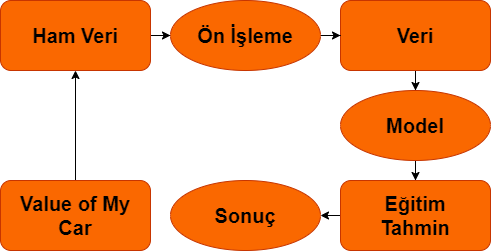
\includegraphics[scale=0.5]{pictures/pic_01.png}&
		\end{tabular}
	\end{center}
	\caption{Value of My Car Akış Diyagramı}
	\label{fig:01}
\end{figure}

Projenin akış diyagramı Şekil \ref{fig:01}'de belirtilmiştir. Makalenin devamında kullanılan algoritmalar ile ilgili bilgiler ve sonuç kısmı bulunmaktadır.

\pagebreak
\section{\textbf{METODLAR}}
\subsection{\textbf{Decision Tree}}

\quad 	Karar ağaçları, genellikle regresyon ve sınıflandırma problemlerinde kullanılır. Ağaç tabanlı algoritmalardan birisi olup karmaşık veri setlerinde kullanılabilir\cite{4}.

\begin{figure}[!h]
	\centering
	\begin{center}
		\begin{tabular}{cc}
			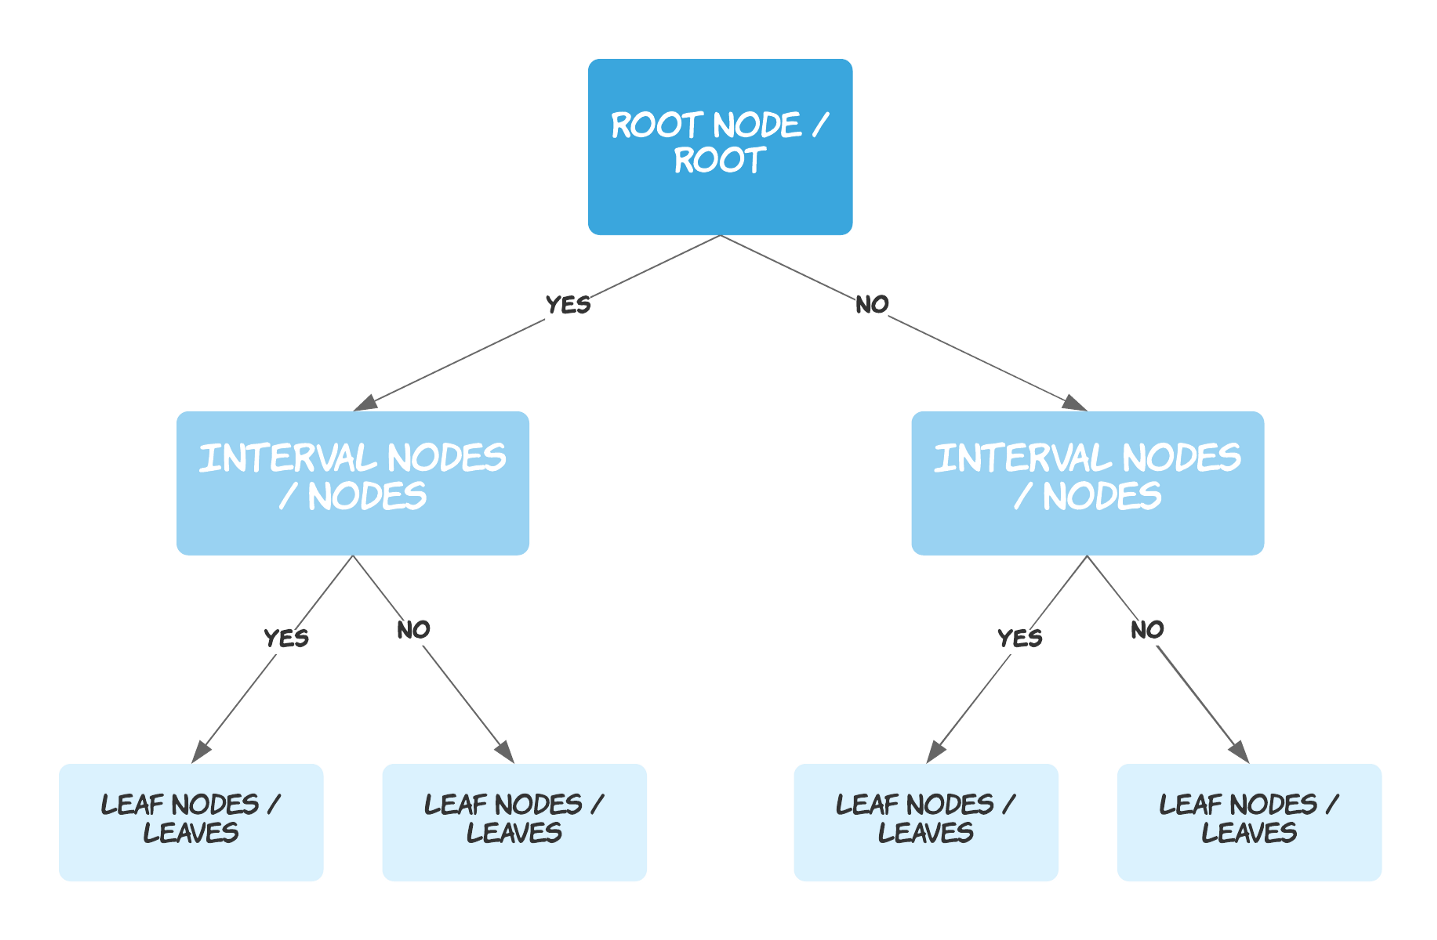
\includegraphics[scale=0.225]{pictures/pic_02.png}&
		\end{tabular}
	\end{center}
	\caption{Decision Tree}
	\label{fig:02}
\end{figure}

\quad Kök (root), karar ağaçlarının ilk basamağına(hücresine) verilen isimdir. Problemimizi gözlemlerken, kök kısmındaki koşullar doğrultusunda sınıflandırma yaparız.

\quad Kök hücrelerin altında düğümler (nodes) vardır. Ele aldığımız her bir gözlemi köklerin aracılığı ile sınıflandırırız. Düğüm sayısının artma oranıyla doğru otantılı bir şekilde, elimizde bulunan modelin karmaşıklığı da artar. Bize sonucu veren yapraklardır ve yapraklar ağacın en altında bulunur\cite{4}.

\quad Kök hücre seçilirken dikkat edilmesi gereken en önemli etken, veri setini iyi açıklayabilmesidir. Köke karar verirken bizim için önemli bazı değerler vardır\cite{4};

\quad Alt kümenin saflık değerine $Gini$ denir. $T$, $pj$, $j$ sınıfının gerçekleşme olasılığını verir. Elimizde bulunan her sınıf için hesaplanır ve elde ettiğimiz sonuçların karesininin toplamını birden çıkartırız. 0 ile 1 arasında bir değere sahiptir ve sonuç 0'a ne kadar yakın olursa o kadar iyi ayrım yapılmıştır denir\cite{4}. 

\quad $Gini$ indexinin formülü Eşitlik \ref{eq:01}'de verilmiştir\cite{15}. Formül değişkenlerinin temsil ettiği veriler de aşağıdaki gibidir;
\begin{itemize}
\item \textbf{$T$:} Tüm veri seti
\item \textbf{$p_{j}$:} Veri setindeki her bir verinin kendinden küçük ve kendinden büyük eleman sayılarına bölümü
\item \textbf{$n$:}  Seçilen verimiz
\end{itemize}

\begin{equation}
\label{eq:01}
\Large Gini(T)=1-\sum_{j=1}^{n}(p_{j})^2
\end{equation}

\pagebreak
\quad Entropy rastgeleliği, belirsizliği ve beklenmeyen durumun ortaya çıkma olasılığını gösterir\cite{5}.  Bu olasılığı $log_{2}$ tabanında yapar\cite{4}.

\begin{equation}
\label{eq:02}
\Large I_{H}=-\sum_{j=1}^{c}p_{j}log_{2}(p_{j})
\end{equation}

\quad Entropi daha dengeli bir ağaç çıkarmaya meyilli iken $Gini$, frekansı fazla olan sınıfı ayrıştırmaya meyillidir.

\subsection{\textbf{Gradient Boosting Regressor}}
\quad Makine öğrenmesi modellerinde doğru tahminleri daha da güçlü bir hale getirmek için Gradient Boosting Regressor kullanılır. Karar ağacı tabanlı algoritmalardan oluşur, yinelemeli olarak çalışırlar. Oluşturulan ağaç yapısı, gelen hatayı en aza indirgeyecek eğilimde olması gerekmektedir. Bu algoritmaları en güçlü kılan bu faktördür\cite{6}.

\quad Gradyan yükseltme algoritmasında en temel amaç, elde edeceğimiz maliyet fonksiyonunu en aza indirebilmek için parametreleri tekrarlamaktır. Ağaç eklerken kaybı en aza indirmek için gradyan iniş prosedürü kullanılır\cite{6}.

Gradyan yükseltme üç unsur içerir:

\begin{itemize}
\item Optimize edilmesi beklenen kayıp fonksiyonun(loss) belirlenmesi. 
\item Optimize edilmiş veride belirlenen zayıf öğrenci ile tahmin yapmak. 
\item Loss’u minimum seviyeye indirgemek için zayıf öğrencilere bir katkı modeli eklenir\cite{7}.
\end{itemize}

\begin{figure}[!h]
	\centering
	\begin{center}
		\begin{tabular}{cc}
			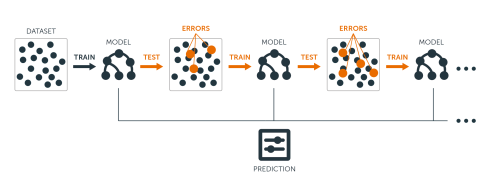
\includegraphics[scale=0.5]{pictures/pic_03.png}&
		\end{tabular}
	\end{center}
	\caption{Gradyan yükseltme algoritması işleyiş süreci\cite{16}}
	\label{fig:03}
\end{figure}

\begin{equation}
\label{eq:03}
\Large Loss^i=\sum_{j=1}^{n}(Y_{j}-F^i(X_{j}))^2
\end{equation}

\pagebreak
\subsection{\textbf{XGB Regressor}}
\quad Gradyan yükseltme algoritmasını çeşitli düzenlemeler ile üstün performanslı haline dönüşmesine denir veya aşırı gradyan artırma olarak da bilinir\cite{9}. Yüksek tahmin gücü elde etmek, boş verileri yönetebilmek ve aşırı öğrenmenin önüne geçmeyi engellemekte oldukça hızlıdır\cite{10}. 

\quad XGB’nin kullanmanın en temel sebebi bulundurduğu kütüphanenin model performansı ve yürütme hızının yüksek olmasına dayanmaktadır\cite{9}.

\quad XGBoost algoritması kullanılırken öncelikle ilk tahmin (base score) yapılmalıdır. Sonraki adımlarda sonuç herhangi bir sayı olabilir. Çünkü yapılacak işlemler yakın sayarak doğru sonuca ulaşacaktır. Sonraki adımda hatalar tahminleyen karar ağacı kurulur. Bu adımdaki amaç hataları öğrenip doğru tahmine yaklaşmaktır. Benzerlik skoru (similarity score) verilerin dallarda ne kadar iyi gruplandığını gösterir. Bu skor oluşturulan ağacın her bir dalı için hesaplanır. 

\begin{equation}
\label{eq:04}
\large Similarity Score=\frac{Sum of Residuals, Squared}{Number of Residuals + \lambda}
\end{equation}

\quad 	Benzerlik skorlarını hesapladıktan sonra elde ettiğimiz sonuçtan daha iyi bir tahmin yapılıp yapılmayacağını öğrenmek için tüm olasılıklardaki ağaçlar kurulur. Hepsi için ayrı ayrı benzerlik skorları hesaplanır ve hangi ağacın daha etkili yani daha iyi olduğunu düzenlemek için Eşitlik \ref{eq:05}'deki kazanç hesabı yapılır\cite{10}. Yukarıda belirttiğimiz benzerlik skorunun sonucu ile dallar değerlendirilirken, elde ettiğimiz Eşitlik \ref{eq:05}'deki kazanç değeri ile ağacın tamamı değerlendirilmektedir\cite{10}.

\begin{equation}
\label{eq:05}
\begin{matrix} Kazanc=SolBenzerlikSkoru+ \\ SagBenzerlikSkoru-OncekiAgacinBenzerlikSkoru \end{matrix}
\end{equation}

\subsection{\textbf{Random Forest}}
\quad Rastgele orman algoritması, denetimli öğrenme algoritması olup hem sınıflandırmada hem de regresyon analizlerinde kullanılır. Aşırı uyumu önler. Random Forest, karar ağaçlarını rastgele bir şekilde oluşturur. İstikrarlı ve doğru bir sonuç tahmini yapabilmek için bunları birleştirir. Ağaç sayısı ve sonuçları arasında doğrudan ilişki bulunmaktadır. Ağaç sayısını ne kadar arttırırsak o kadar kesin bir sonuç elde ederiz\cite{11}\cite{12}.

\begin{figure}[!h]
	\centering
	\begin{center}
		\begin{tabular}{cc}
			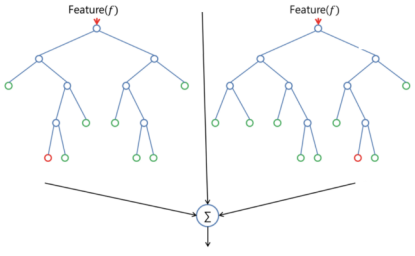
\includegraphics[scale=0.65]{pictures/pic_04.png}&
		\end{tabular}
	\end{center}
	\caption{Random Forest\cite{12}}
	\label{fig:04}
\end{figure}

\quad Rastgele orman algoritması, ağaç büyütme aşamasında, normal durumun üzerine rastgelelik durumunu da kullanıyor\cite{12}.

\pagebreak
\subsection{\textbf{LightGBM Regressor}}
\quad LightGBM, histogram tabanı kullanan bir algoritmadır. Sürekli verileri giriş olarak alır, bu verileri kesikli hale getirir. Bunu yapmasındaki amaç maliyeti azaltmaktır. Karar ağacı algoritmasının bölünmesi ile doğru orantılıdır. Veriyi optimize etmesi, eğitim süresini düşürür ve daha az kaynak kullanılmasını sağlar\cite{13}.

\quad Karar ağacı algoritmasında yaprak ve seviye olarak iki farklı strateji kullanılabilir. Yaprak stratejisinde kayıp oranını azaltan yapraklar üzerinden bölünme işlemi devam eder. Seviye stratejisinde hedeflenen durum ise ağaç büyütülürken dengesini korumaktır. Yaprak stratejisinde hatayı minimize etmek amaçlandığı için, seviye stratejisine göre daha düşük hata oranına sahiptir. Bunun etkilediği durumlardan biri de öğrenme aşamasının hızlanmasıdır. Bu yüzden, boosting algoritmalarının geri kalanından ayrılır. Elimizde bulunan veri sayısı ne kadar çoksa, yaprak stratejisini kullanmak o kadar mantıklı olur. Aşırı öğrenmeye sebebiyet vermemek için veri sayısının az olduğu durumlarda kullanıma uygun değildir. Bu durumda da seviye stratejisi kullanılır\cite{13}.

\begin{figure}[!h]
	\centering
	\begin{center}
		\begin{tabular}{cc}
			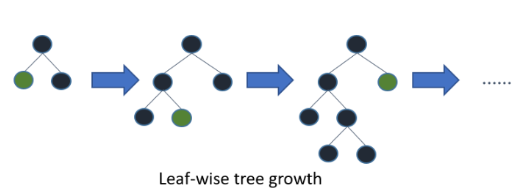
\includegraphics[scale=0.5]{pictures/pic_05.png}&
		\end{tabular}
	\end{center}
	\caption{Yaprak odaklı(leaf wise) strateji\cite{13}}
	\label{fig:05}
\end{figure}

\begin{figure}[!h]
	\centering
	\begin{center}
		\begin{tabular}{cc}
			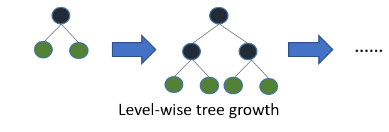
\includegraphics[scale=0.5]{pictures/pic_06.png}&
		\end{tabular}
	\end{center}
	\caption{Seviye odaklı(level wise) strateji\cite{13}}
	\label{fig:06}
\end{figure}
\pagebreak

\subsection{\textbf{CatBoost Regressor}}
\quad Gradient Boosting tabanlı açık kaynak kodlu bir makine öğrenmesi algoritmasıdır. Veri hazırlığı süresini düşürdüğü için önemli bir yere sahiptir. Elinde bulunan boş veriler ile baş edebilir ancak kategorik veriler için kodlamaya ihtiyaç duyar. Yüksek öğrenme hızı, sayısal, kategorik ve metin verileri ile çalışabilmesi en belirgin özelliklerindendir. Ayrıca aşırı öğrenme sorununu ortadan kaldırmak için simetrik ağaç kurar. Over-fitting (aşırı öğrenme) durumunun oluşması durumunda, belirlenen özelliklere varmadan önce öğrenme işlemi durdurulur\cite{14}.

\begin{figure}[!h]
	\centering
	\begin{center}
		\begin{tabular}{cc}
			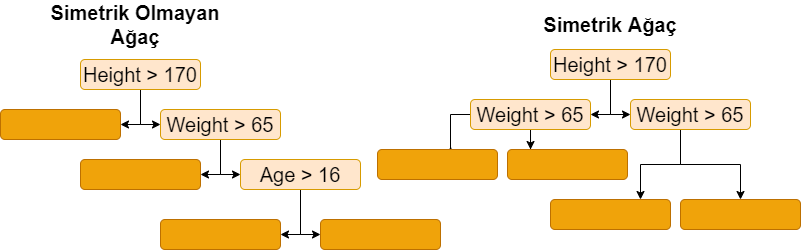
\includegraphics[scale=0.325]{pictures/pic_07.png}&
		\end{tabular}
	\end{center}
	\caption{Simetrik/Simetrik olmayan ağaç}
	\label{fig:07}
\end{figure}

\section{\textbf{SONUÇLAR}}

\quad Veri setimizdeki verilerin \%70'ini eğitim, \%30'unu ise test verisi olarak ayırdık. Daha sonra ayırdığımız verileri, algoritmalarımızın eğitim ve tahmin aşamalarında kullandık. Bu aşamalar sonucunda elde ettiğimiz doğruluk değerlerine Şekil \ref{fig:08}'de, $MSE$ (ortalama kare hatası) değerlerine de Şekil \ref{fig:09}'da yer verdik.

\begin{figure}[!h]
	\centering
	\begin{center}
		\begin{tabular}{cc}
			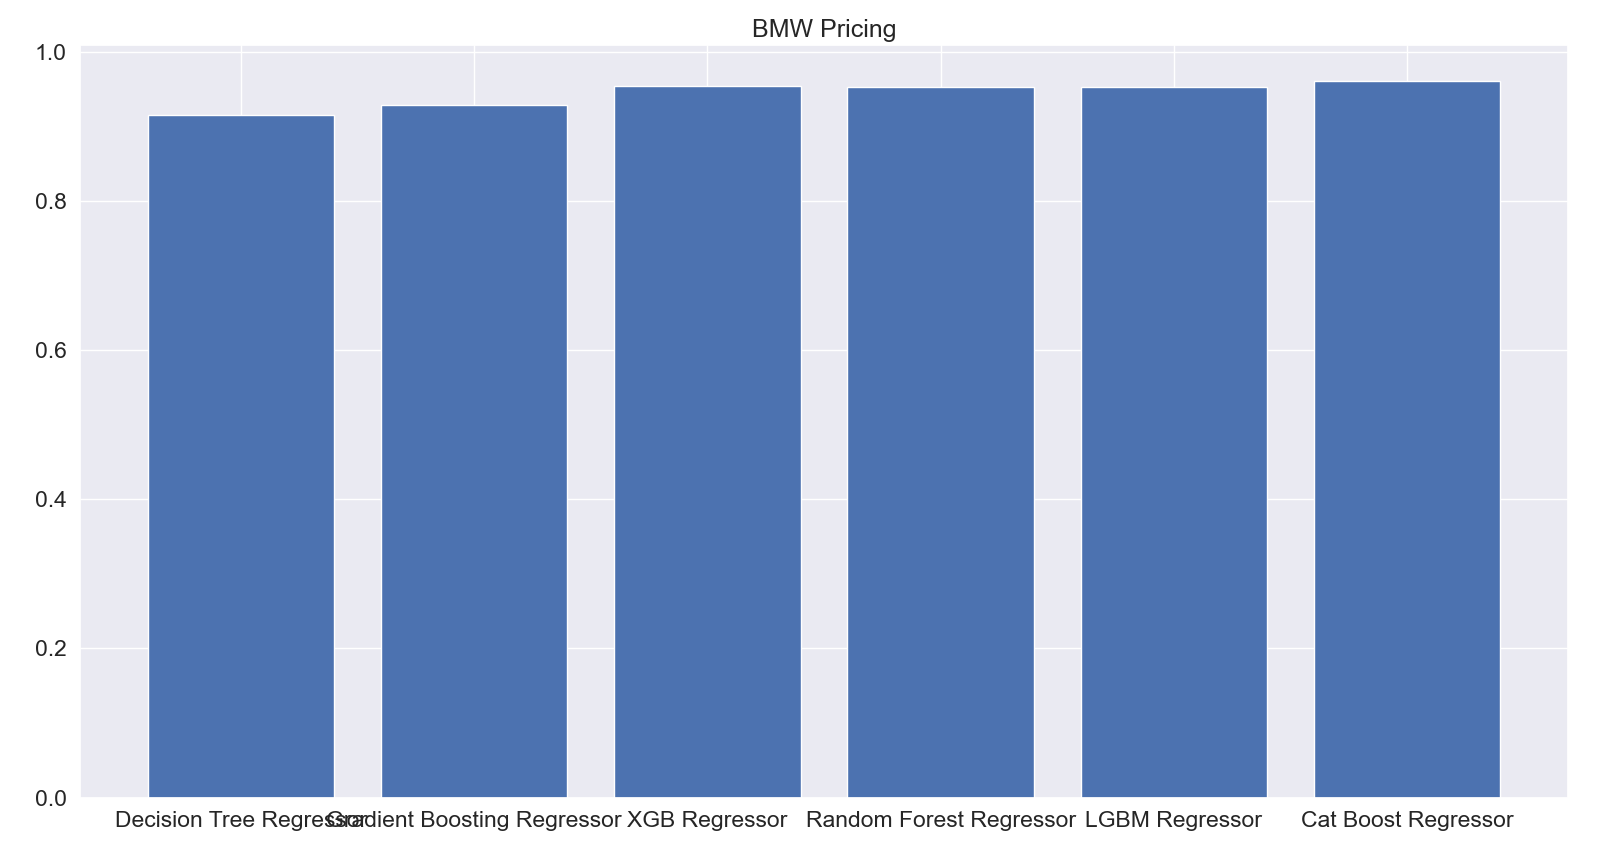
\includegraphics[scale=0.175]{pictures/pic_08.png}&
		\end{tabular}
	\end{center}
	\caption{Tüm Algoritmaların Doğruluk $(r2)$ Değerleri}
	\label{fig:08}
\end{figure}

\begin{figure}[!h]
	\centering
	\begin{center}
		\begin{tabular}{cc}
			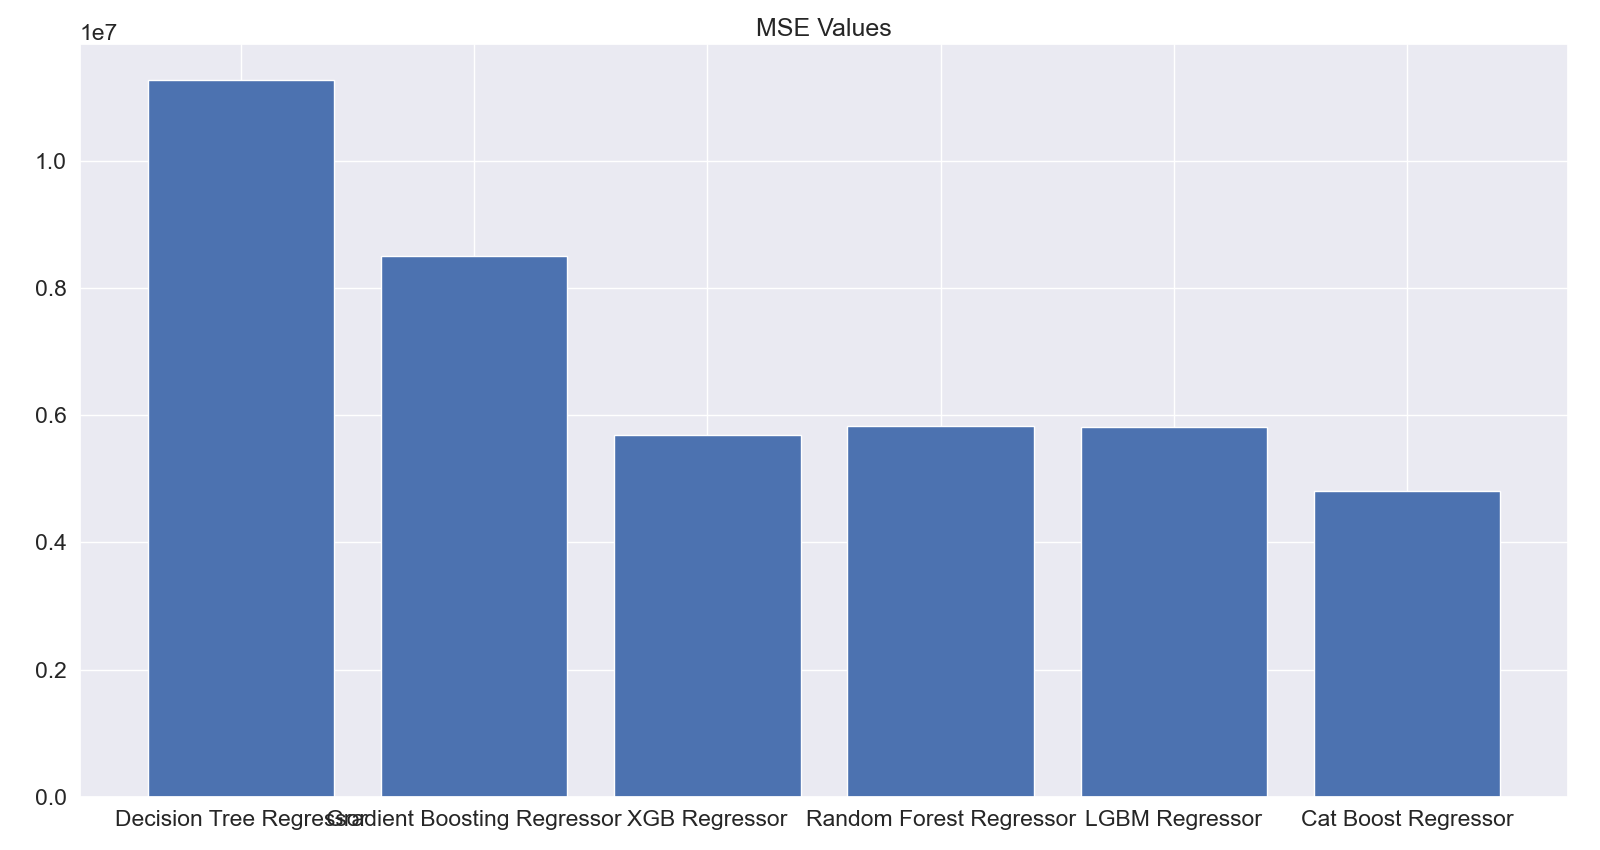
\includegraphics[scale=0.175]{pictures/pic_09.png}&
		\end{tabular}
	\end{center}
	\caption{Tüm Algoritmaların $MSE$ Değerleri}
	\label{fig:09}
\end{figure}

\quad İkinci el araç fiyatlarının tahmin edilebilmesi için "100.000 UK Used Car" \cite{3} veri setindeki "BMW.csv" verisini aldık. DT, GB, XGB, RF, LGBM ve CB regressor algoritmalarını kullandık. Bu algoritmaların $r2$ ve $MSE$ değerleri Tablo \ref{tbl:01}'de yer almaktadır.

\begin{table}[h]
	\centering
	\normalsize
	\begin{tabular}{|l|c|c|c|c|}
		\hline
					& \textbf{r2}	& \textbf{MSE}	\\ \hline
		\textbf{DT}		& 0.9209		& 0.0825		\\ \hline
		\textbf{GB}		& 0.9296		& 0.0657		\\ \hline
		\textbf{XGB}		& 0.9538		& 0.0447		\\ \hline
		\textbf{RF}		& 0.9533		& 0.0453		\\ \hline
		\textbf{LGBM}	& 0.9533		& 0.0449		\\ \hline
		\textbf{CB}		& \textbf{0.9614}	& \textbf{0.0372}	\\ \hline
	\end{tabular}
	\caption{DT, GB, XGB, RF, LGBM ve CB regressor algoritmalarının $r2$ ve $MSE$ degerleri}
	\label{tbl:01}
\end{table}

\quad Tablo \ref{tbl:01}'i incelersek, en yüksek doğruluk değerinin $\%96.14$ oranıyla CatBoost algoritmasına ait olduğunu görebiliriz. Aynı zamanda en düşük $MSE$ değeri de $0.0372$ oranıyla yine CatBoost'a ait. Bu verilerden en düşük doğruluk değerine sahip olan algoritma ise Decision Tree$(\%92.09)$'dur. $r2$ ve $MSE$ değerlerinin arasındaki ters orantıdan dolayı, en yüksek $MSE$ değeri yine Decision Tree$(0.0825)$'e aittir. Diğer algoritmaların $r2$ ve $MSE$ değerlerini de Tablo \ref{tbl:01} üzerinde inceleyebiliriz.


\subsection{\textbf{Cross-Validation (Çapraz Doğrulama)}}
\quad Regresyon algoritmalarımız birer kez eğitildi ve test edildi. Bu eğitimlerin sonuçlarını da Tablo \ref{tbl:01}'de belirttik. Şimdi  DT, GB, XGB, RF, LGBM ve CB regressor algoritmalarımızı \textbf{Cross-Validation} metoduyla 30 kez rastgele olacak şekilde çalıştırdık ve sonuçları Şekil \ref{fig:10}, \ref{fig:11}, \ref{fig:12}, \ref{fig:13}, \ref{fig:14} ve \ref{fig:15}'de verdik.

\begin{figure}[!h]
	\centering
	\begin{center}
		\begin{tabular}{cc}
			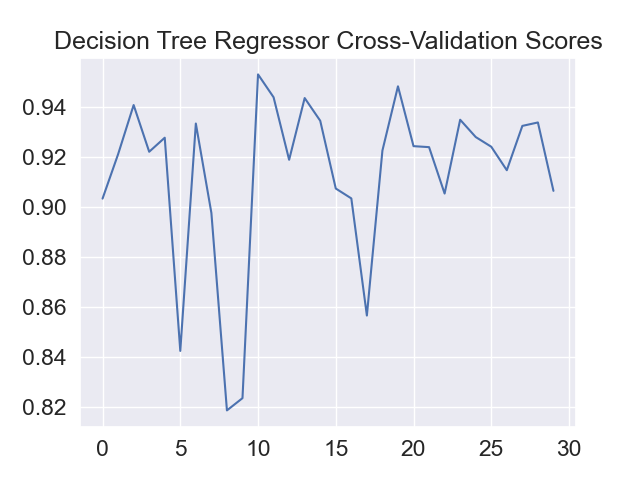
\includegraphics[scale=0.5]{pictures/pic_10.png}&
		\end{tabular}
	\end{center}
	\caption{Decision Tree Regressor Cross-Validation}
	\label{fig:10}
\end{figure}
\pagebreak
\begin{figure}[!h]
	\centering
	\begin{center}
		\begin{tabular}{cc}
			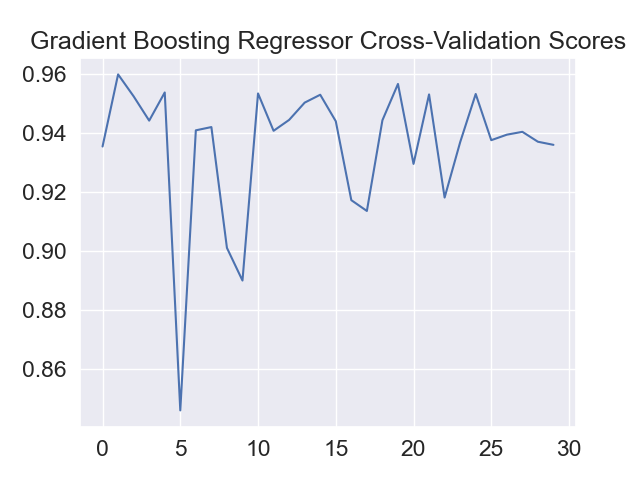
\includegraphics[scale=0.5]{pictures/pic_11.png}&
		\end{tabular}
	\end{center}
	\caption{Gradient Boost Regressor Cross-Validation}
	\label{fig:11}
\end{figure}

\begin{figure}[!h]
	\centering
	\begin{center}
		\begin{tabular}{cc}
			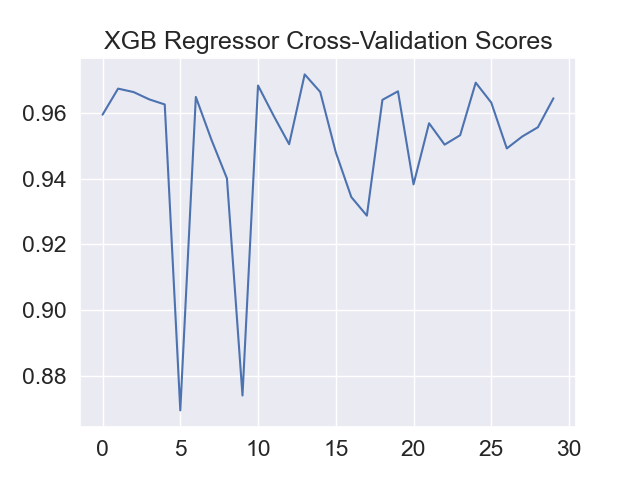
\includegraphics[scale=0.5]{pictures/pic_12.png}&
		\end{tabular}
	\end{center}
	\caption{XGB Regressor Cross-Validation}
	\label{fig:12}
\end{figure}

\begin{figure}[!h]
	\centering
	\begin{center}
		\begin{tabular}{cc}
			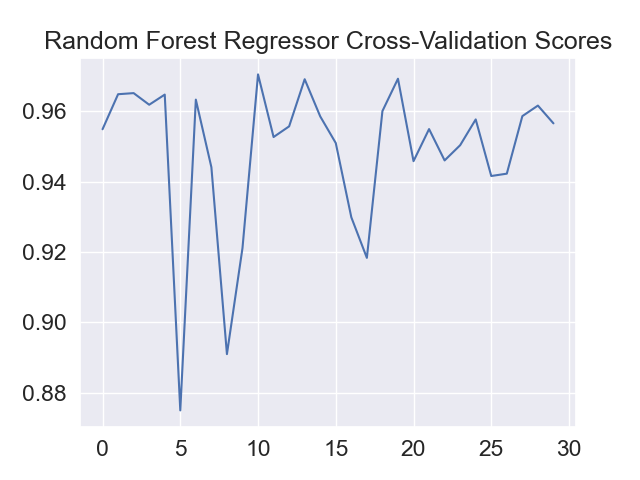
\includegraphics[scale=0.5]{pictures/pic_13.png}&
		\end{tabular}
	\end{center}
	\caption{Random Forest Regressor Cross-Validation}
	\label{fig:13}
\end{figure}
\pagebreak
\begin{figure}[!h]
	\centering
	\begin{center}
		\begin{tabular}{cc}
			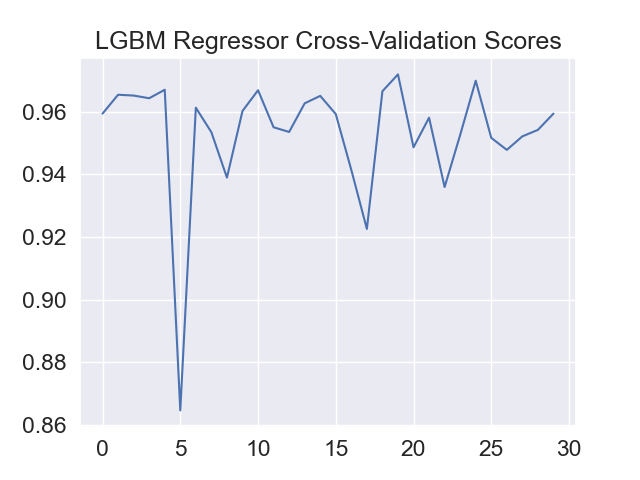
\includegraphics[scale=0.5]{pictures/pic_14.png}&
		\end{tabular}
	\end{center}
	\caption{LGBM Regressor Cross-Validation}
	\label{fig:14}
\end{figure}

\begin{figure}[!h]
	\centering
	\begin{center}
		\begin{tabular}{cc}
			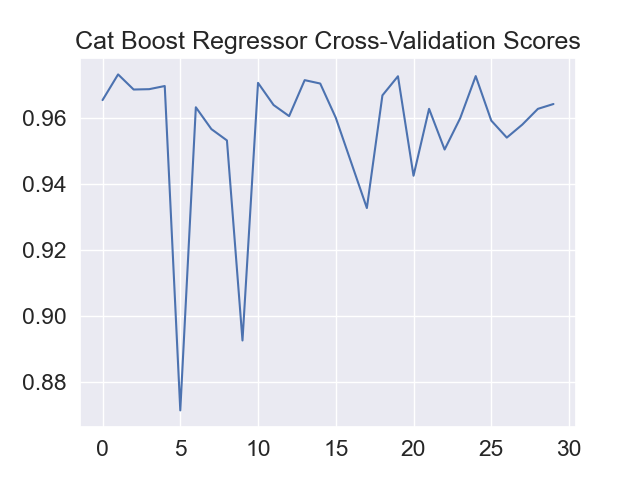
\includegraphics[scale=0.5]{pictures/pic_15.png}&
		\end{tabular}
	\end{center}
	\caption{CatBoost Regressor Cross-Validation}
	\label{fig:15}
\end{figure}

\quad Bu algoritmaların Cross-Validaion sonuçlarının ortalamaları Şekil \ref{fig:16}'daki gibidir. Bu değerler aynı zamanda Tablo \ref{tbl:02}'de de sayısal olarak yer almakta.

\begin{figure}[!h]
	\centering
	\begin{center}
		\begin{tabular}{cc}
			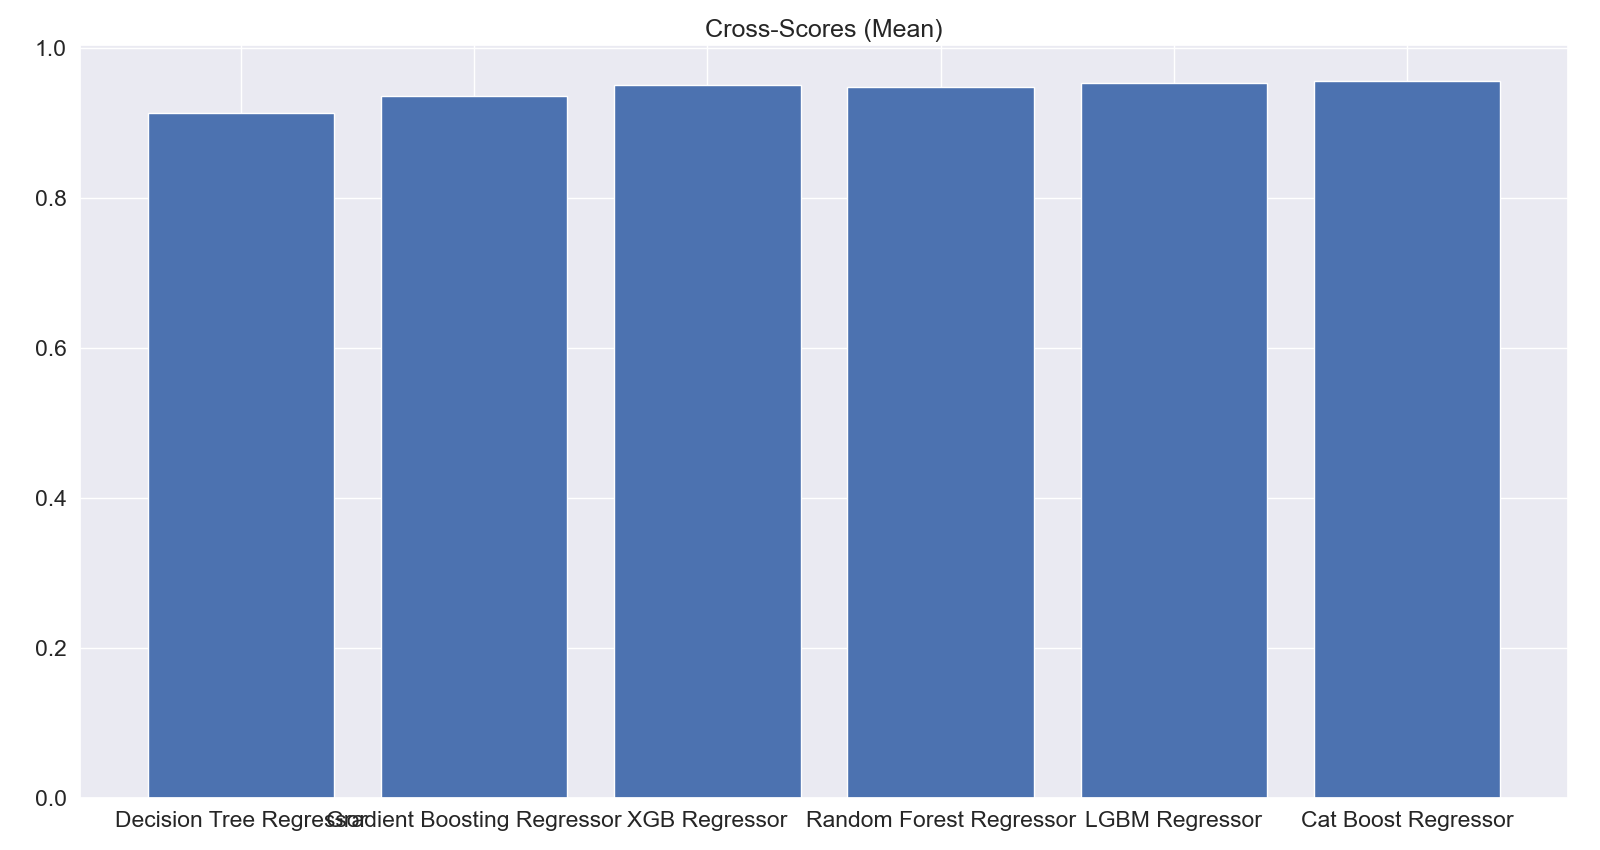
\includegraphics[scale=0.2]{pictures/pic_16.png}&
		\end{tabular}
	\end{center}
	\caption{Cross-Validation Ortalama(Mean) Değerleri}
	\label{fig:16}
\end{figure}
\pagebreak
\begin{table}[h]
	\centering
	\normalsize
	\begin{tabular}{|l|c|c|c|c|}
		\hline
					& \textbf{Cross-Validation Score(mean)}	\\ \hline
		\textbf{DT}		& 0.9160		\\ \hline
		\textbf{GB}		& 0.9356		\\ \hline
		\textbf{XGB}		& 0.9512		\\ \hline
		\textbf{RF}		& 0.9485		\\ \hline
		\textbf{LGBM}	& 0.9531		\\ \hline
		\textbf{CB}		& \textbf{0.9562}	\\ \hline
	\end{tabular}
	\caption{DT, GB, XGB, RF, LGBM ve CB regressor algoritmalarının Cross-Validation sonuçlarının ortalama(mean) degerleri}
	\label{tbl:02}
\end{table}

\quad Tablo \ref{tbl:02}'yi incelersek, en yüksek doğruluk değerinin $\%95.62$ oranıyla CatBoost algoritmasına ait olduğunu görebiliriz. Bu verilerden en düşük doğruluk değerine sahip olan algoritma ise Decision Tree$(\%91.60)$'dır. Diğer algoritmaların Cross-Validation sonuçlarının ortalama değerlerini de Tablo \ref{tbl:02} üzerinde inceleyebiliriz.

\subsection{\textbf{Valid Data-Pred Data$(Diff)$}}

\begin{figure}[!h]
	\centering
	\begin{center}
		\begin{tabular}{cc}
			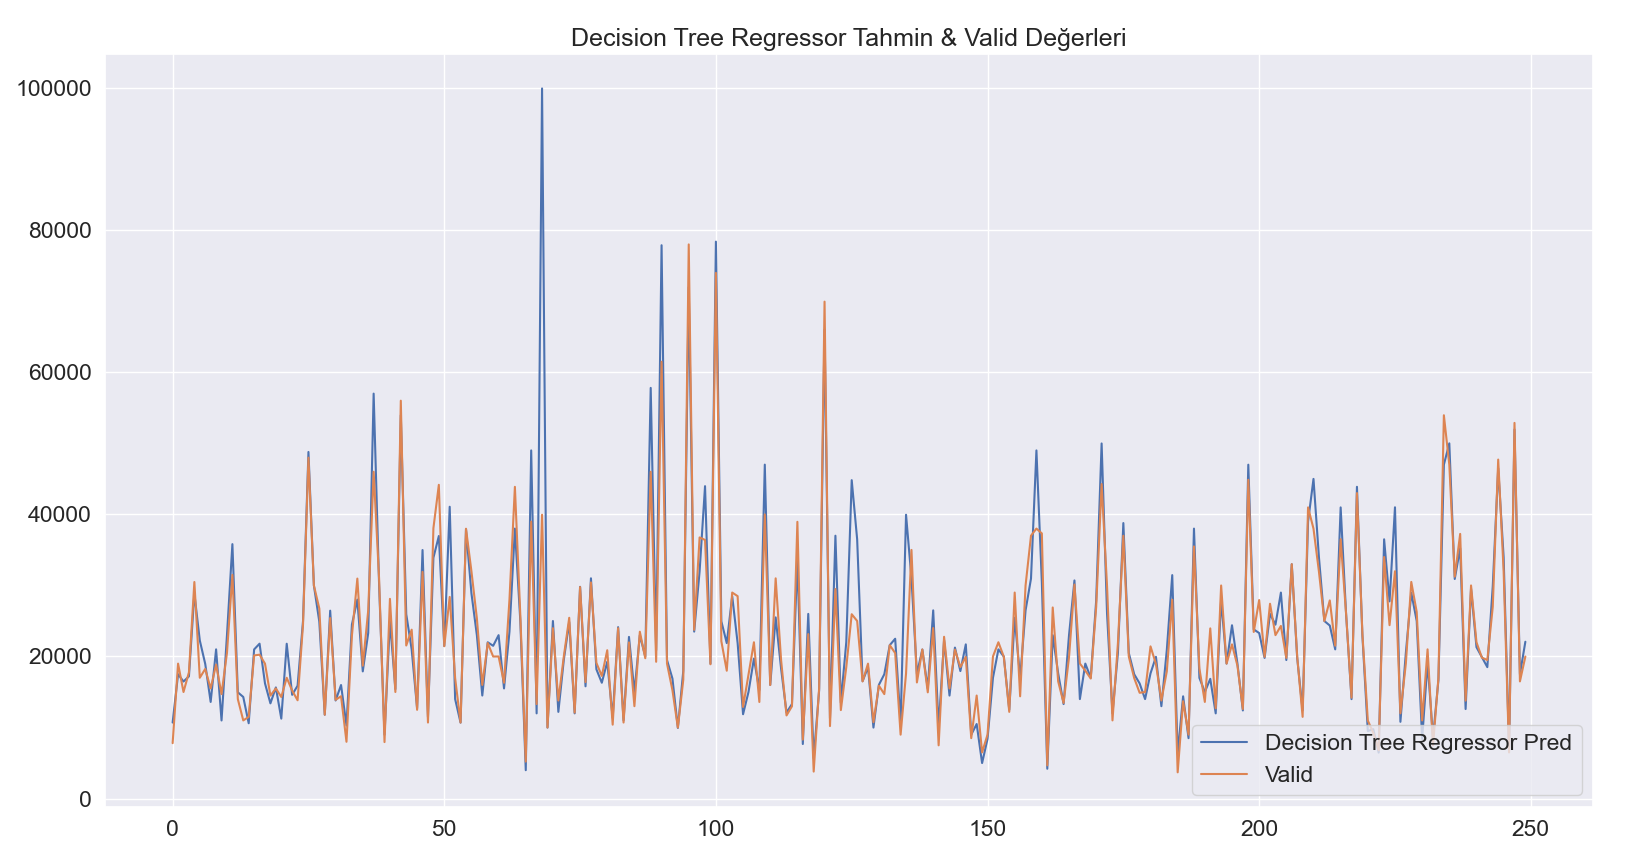
\includegraphics[scale=0.2]{pictures/pic_17.png}&
		\end{tabular}
	\end{center}
	\caption{Decision Tree Regressor Tahmin \& Valid Değerleri}
	\label{fig:17}
\end{figure}

\begin{figure}[!h]
	\centering
	\begin{center}
		\begin{tabular}{cc}
			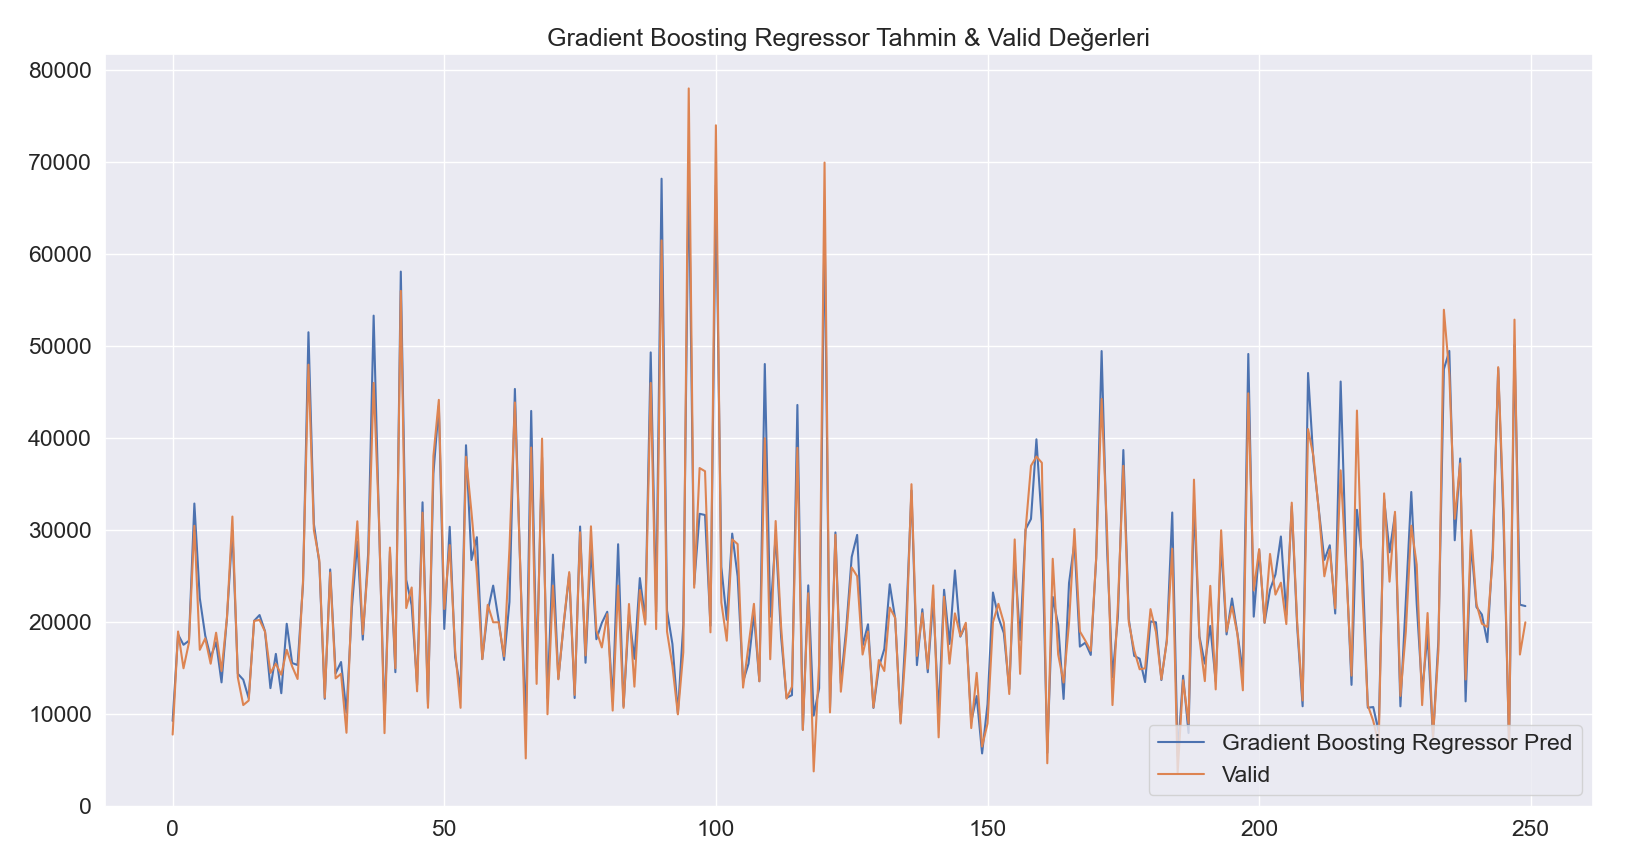
\includegraphics[scale=0.2]{pictures/pic_18.png}&
		\end{tabular}
	\end{center}
	\caption{Gradient Boosting Regressor Tahmin \& Valid Değerleri}
	\label{fig:18}
\end{figure}
\pagebreak
\begin{figure}[!h]
	\centering
	\begin{center}
		\begin{tabular}{cc}
			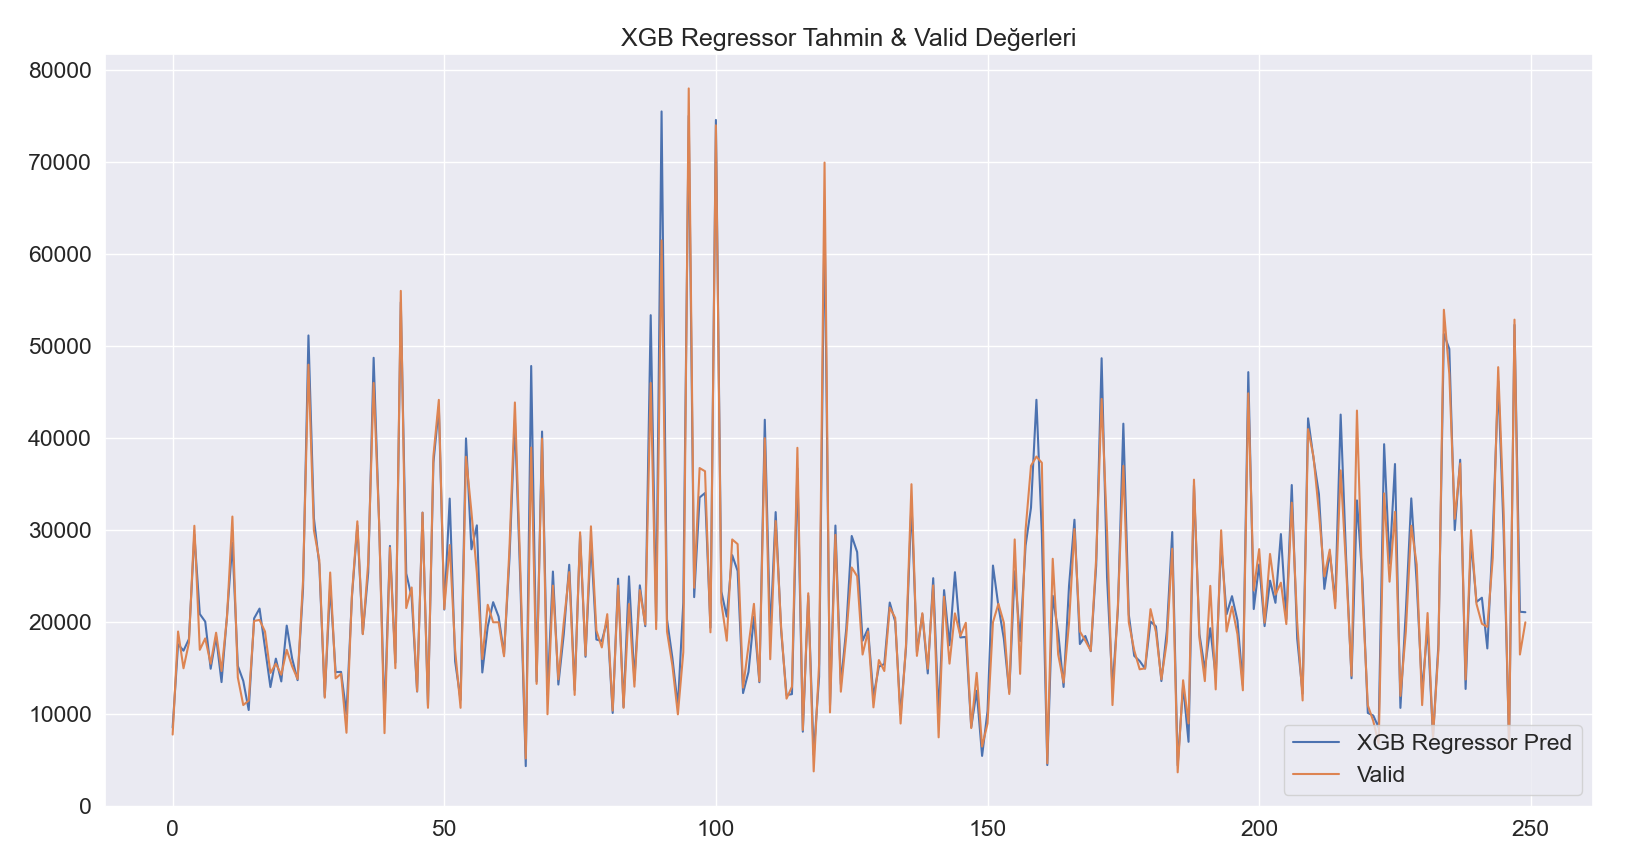
\includegraphics[scale=0.18]{pictures/pic_19.png}&
		\end{tabular}
	\end{center}
	\caption{XGB Regressor Tahmin \& Valid Değerleri}
	\label{fig:19}
\end{figure}

\begin{figure}[!h]
	\centering
	\begin{center}
		\begin{tabular}{cc}
			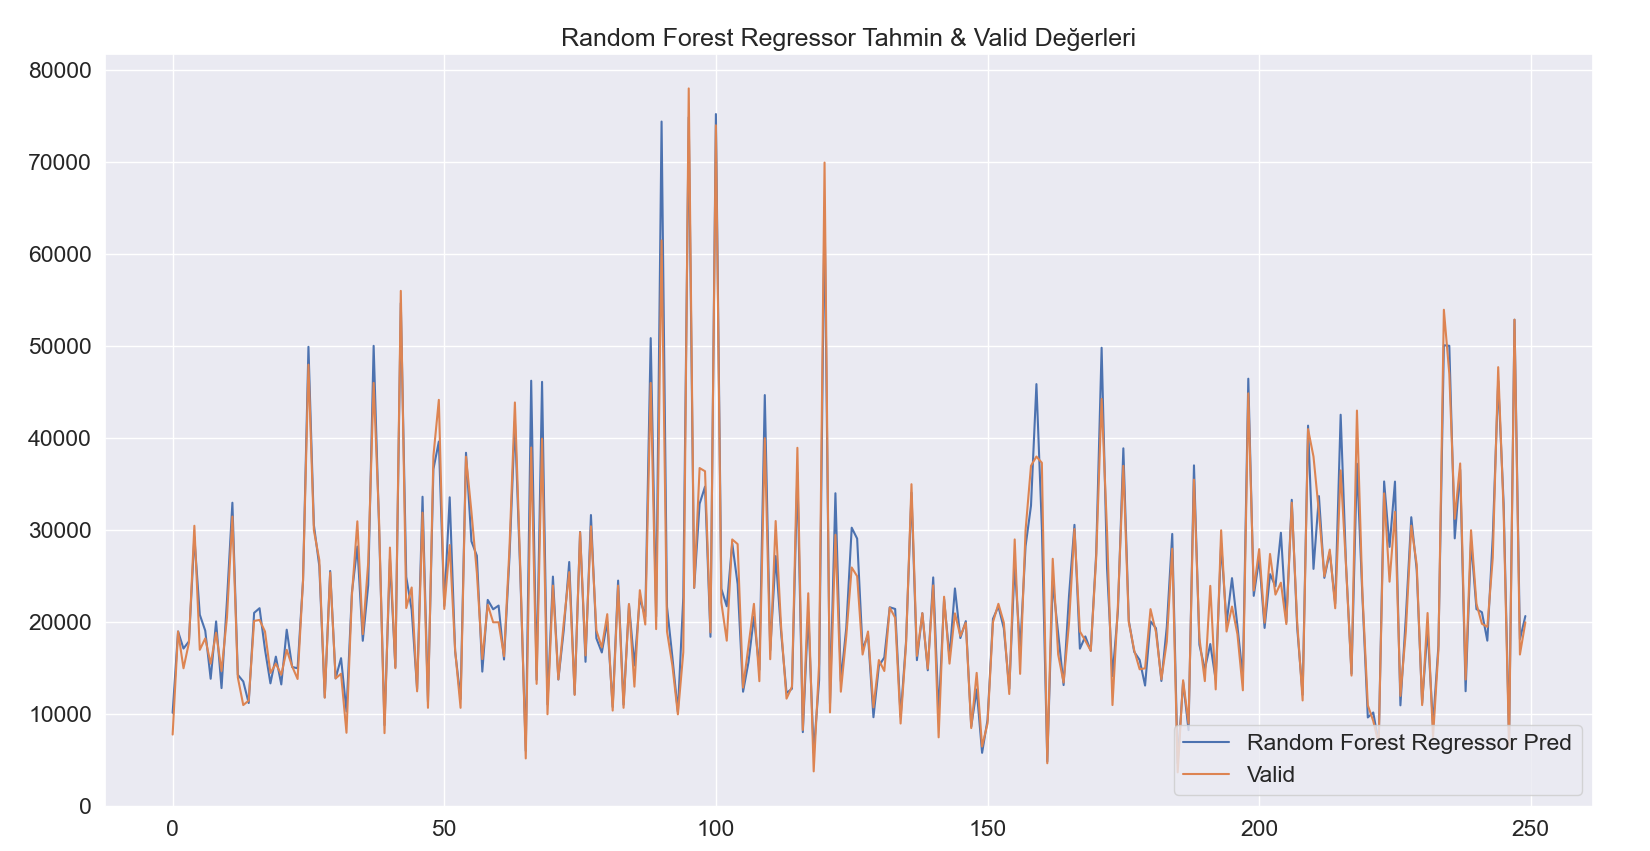
\includegraphics[scale=0.18]{pictures/pic_20.png}&
		\end{tabular}
	\end{center}
	\caption{Random Forest Regressor Tahmin \& Valid Değerleri}
	\label{fig:20}
\end{figure}

\begin{figure}[!h]
	\centering
	\begin{center}
		\begin{tabular}{cc}
			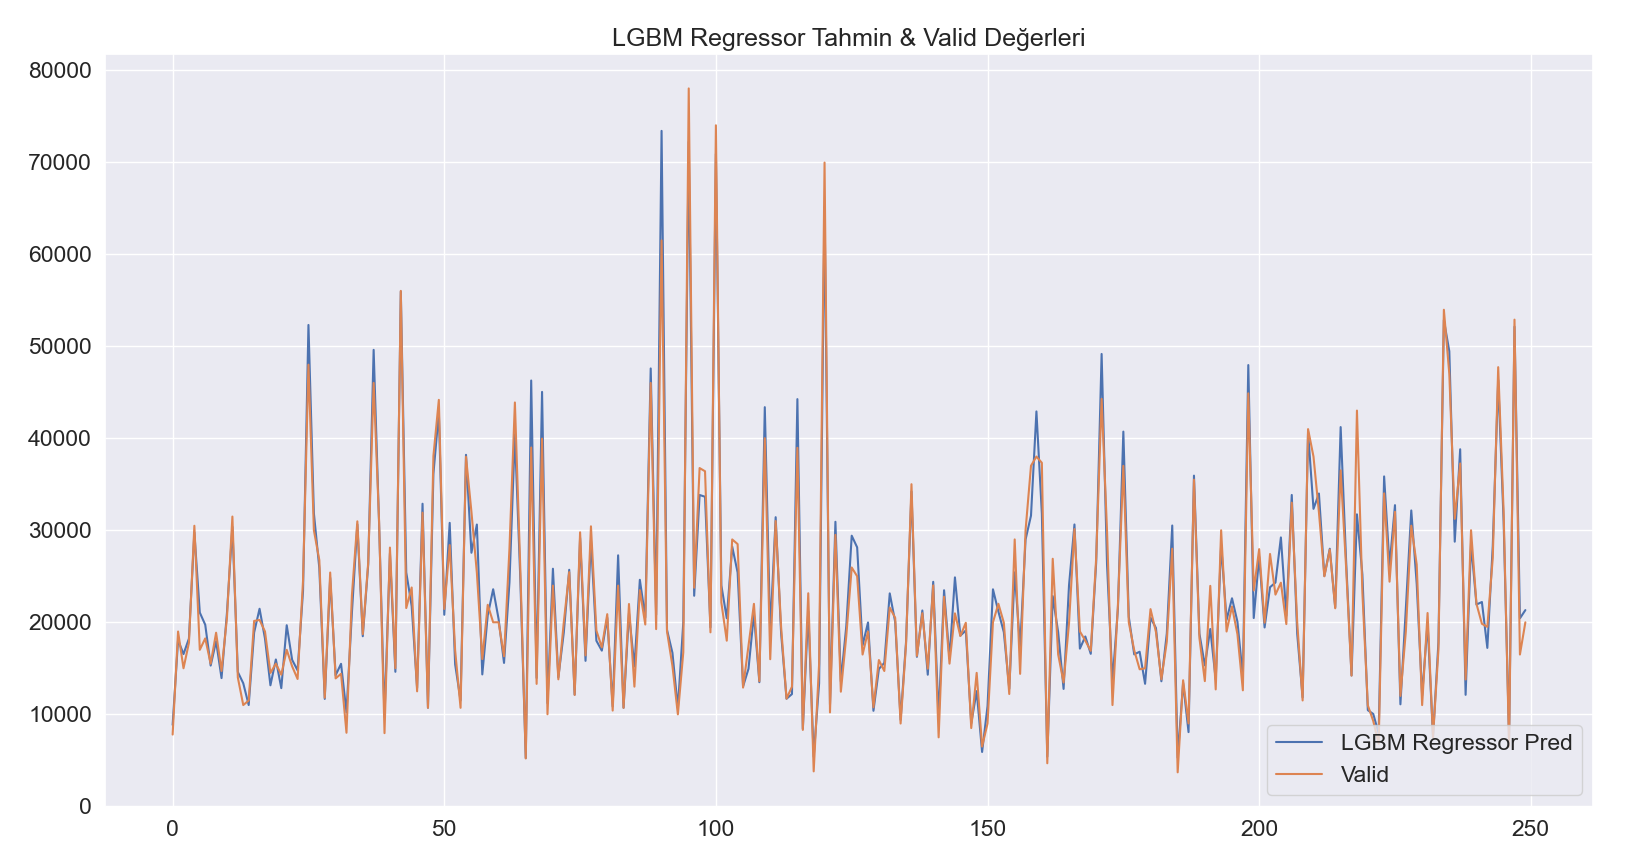
\includegraphics[scale=0.18]{pictures/pic_21.png}&
		\end{tabular}
	\end{center}
	\caption{LGBM Regressor Tahmin \& Valid Değerleri}
	\label{fig:21}
\end{figure}

\begin{figure}[!h]
	\centering
	\begin{center}
		\begin{tabular}{cc}
			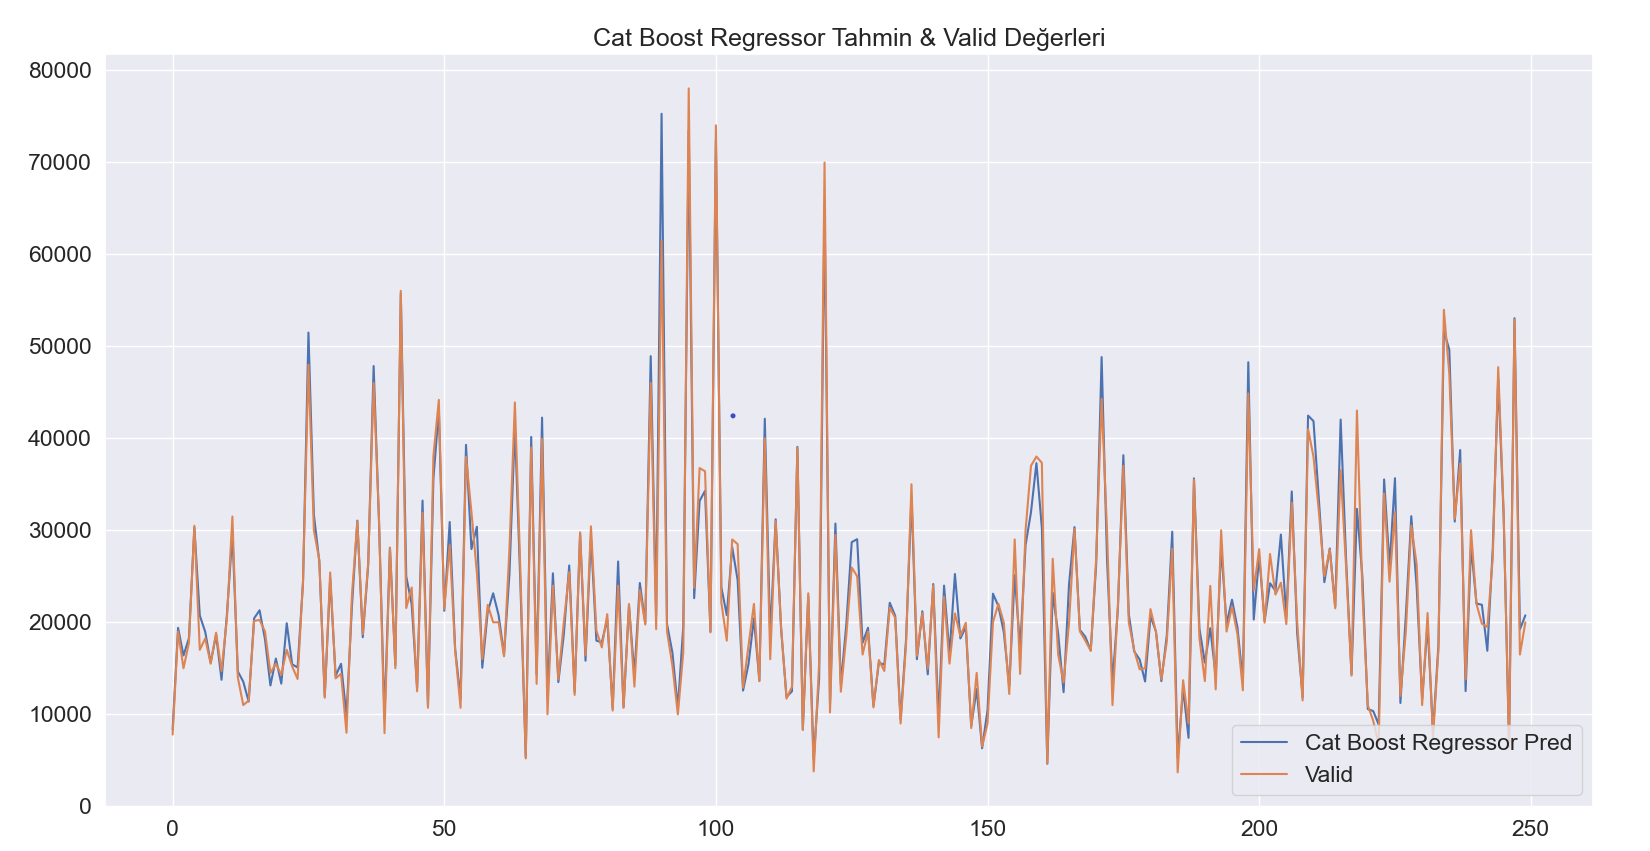
\includegraphics[scale=0.18]{pictures/pic_22.png}&
		\end{tabular}
	\end{center}
	\caption{CatBoost Regressor Tahmin \& Valid Değerleri}
	\label{fig:22}
\end{figure}
\pagebreak

\quad Şekil \ref{fig:17}, \ref{fig:18}, \ref{fig:19}, \ref{fig:20}, \ref{fig:21} ve \ref{fig:22}'de de gösterildiği gibi; gerçek $(valid)$ verilerimiz turuncu, algoritmanın tahmin $(predict)$ değerleri ise mavi hatla gösterilmiştir. Bu grafikler oluşturulurken amacımız; tahmin verisinin gerçek veriden ne kadar saptığını(uzaklaştığını) görmektir.

\section{\textbf{SONUÇ}}

\quad Bu projede kullandığımız veri seti sayesinde ikinci el araçların, değerinin altında veya üstünde bir fiyata satılması yerine, olması gereken fiyatta satılmasını sağlamak için; yapay zeka kullanarak fiyat tahmini yapmaya çalıştık. Tahmin işlemini, daha önceden belirlenen algoritmaları kullanarak yaptık. Algoritmaları, makalenin önceki başlıklarında da anlattığımız çeşitli işlemlere tâbi tutarak bazı sonuçlar elde ettik. Bu sonuçları karşılaştırdık ve en iyi agoritmayı bulmaya çalıştık. Elimizdeki veri setiyle en uyumlu çalışan algoritmayı bulduk ve raporladık. Eğitim sonuçlarını daha yüksek oranlara taşımak için de veri seti optimize edilebilir, gerekli öznitelikler eklenebilir veya gereksiz olanlar çıkartılabilir. Bu sayede daha doğru bir tahminleme işlemi yapabiliriz.

\begin{figure}[!h]
	\centering
	\begin{center}
		\begin{tabular}{cc}
			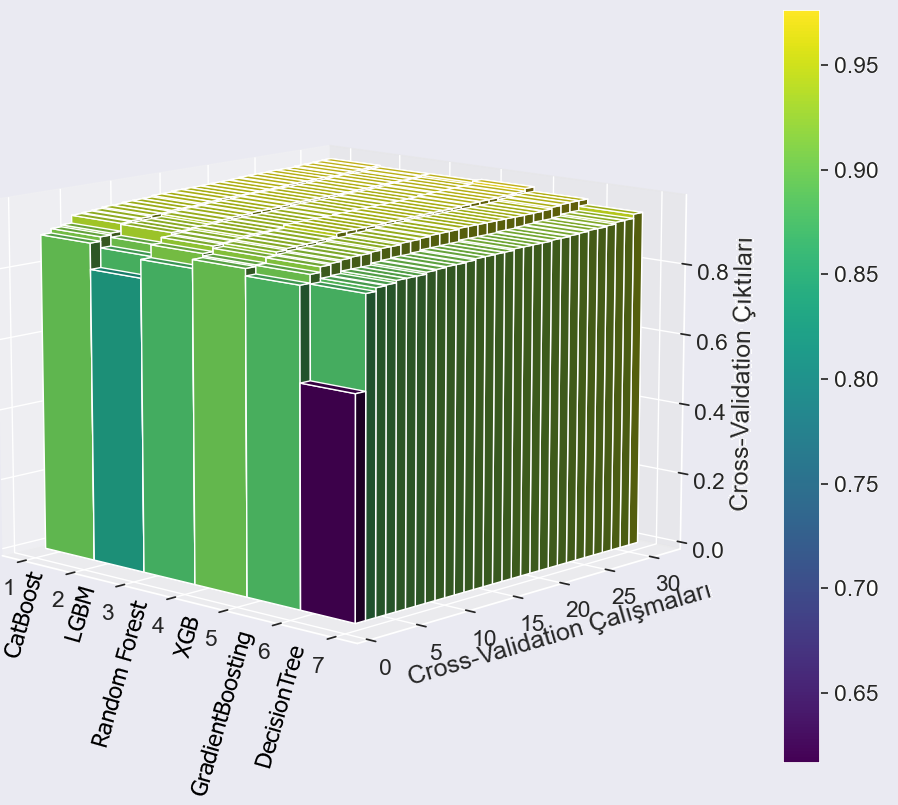
\includegraphics[scale=0.35]{pictures/pic_23.png}&
		\end{tabular}
	\end{center}
	\caption{Algoritmaların Cross-Validation Sonuçları (3D Grafik)}
	\label{fig:23}
\end{figure}

\quad $X$ eksenine baktığımız zaman algoritmaları, $Y$ eksenine baktığımız zaman algoritmaların çalışma sayılarını görüyoruz. Daha sonradan 3. boyuta ise bu çalışmaların skorları $Z$ ekseni olarak ekleniyor ve Şekil \ref{fig:23}'deki 3D grafiği elde ediyoruz. Algoritmalar ve çalışma skorları kendi arasında sıralı olduğu için, sütunlara çapraz açıdan bakıldığında en verimli algoritmanın en yüksekte kaldığını görebiliriz.

\newpage
%%%%%%%%%%%%%%%%%%%%
\newpage
\begin{thebibliography}{16}

\bibitem{1}
DergiPark - İkinci El Otomobil Talep Fiyatının Regresyon Analizi
\\\texttt{\href{https://dergipark.org.tr/tr/download/article-file/431769}{\nolinkurl{dergipark.org.tr/article-file/431769}}}

\bibitem{2}
IjcaOnline - Vehicle Price Prediction
\\\texttt{\href{https://www.ijcaonline.org/archives/volume167/number9/noor-2017-ijca-914373.pdf}{\nolinkurl{ijcaonline.org/archives/noor-2017-ijca-914373}}}

\bibitem{3}
Kaggle - 100.000 UK Used Car Data Set
\\\texttt{\href{https://www.kaggle.com/adityadesai13/used-car-dataset-ford-and-mercedes?select=bmw.csv}{\nolinkurl{kaggle.com/adityadesai13/used-car-dataset-bmw}}}

\bibitem{4}
Medium - Karar Ağaçları
\\\texttt{\href{https://medium.com/deep-learning-turkiye/karar-ağaçları-makine-öğrenmesi-serisi-3-a03f3ff00ba5}{\nolinkurl{medium.com/deep-learning/karar-ağaçlari}}}

\bibitem{5}
Başkent - Karar Ağacı
\\\texttt{\href{http://mail.baskent.edu.tr/~20410964/DM_8.pdf}{\nolinkurl{baskent.edu.tr/20410964/DM_8.pdf}}}

\bibitem{6}
Data Science - Boosting Algoritmaları
\\\texttt{\href{https://www.datasciencearth.com/boosting-algoritmalari/}{\nolinkurl{datasciencearth.com/boosting-algoritmalari}}}

\bibitem{7}
Tevfik Bulut - Gradyan Yükseltme Algoritması
\\\texttt{\href{https://tevfikbulut.com/2020/06/27/topluluk-ogrenme-algoritmalarindan-gradyan-yukseltme-algoritmasi-ile-gogus-kanserinin-tahmini-uzerine-bir-vaka-calismasi-a-case-study-on-the-prediction-of-breast-cancer-using-gradient-boosting-algori/}{\nolinkurl{tevfikbulut.com/prediction-of-breast-cancer}}}

\bibitem{8}
OpenGenus - Boosting Algorithms
\\\texttt{\href{https://iq.opengenus.org/types-of-boosting-algorithms/}{\nolinkurl{opengenus.org/types-of-boosting-algorithms}}}

\bibitem{9}
OpenGenus - XGBoost
\\\texttt{\href{https://iq.opengenus.org/xgboost/}{\nolinkurl{opengenus.org/xgboost}}}

\bibitem{10}
Veri Bilimi Okulu  - XGBoost Nasıl Çalışır
\\\texttt{\href{https://www.veribilimiokulu.com/xgboost-nasil-calisir/}{\nolinkurl{veribilimiokulu.com/xgboost-nasil-calisir}}}

\bibitem{11}
Medium - Rastgele Orman Algoritması
\\\texttt{\href{https://medium.com/@cemthecebi/rastgele-orman-algoritması-1600ca4f4784}{\nolinkurl{medium.com/@cemthecebi/rastgele-orman}}}

\bibitem{12}
DevHunter - Rastgele Orman Algoritması
\\\texttt{\href{https://devhunteryz.wordpress.com/2018/09/20/rastgele-ormanrandom-forest-algoritmasi/comment-page-1/}{\nolinkurl{devhunteryz.wordpress.com/random-forest}}}

\bibitem{13}
Veri Bilimi Okulu - LightGBM
\\\texttt{\href{https://www.veribilimiokulu.com/lightgbm/}{\nolinkurl{veribilimiokulu.com/lightgbm}}}

\bibitem{14}
Veri Bilimi Okulu - CatBoost Nedir
\\\texttt{\href{https://www.veribilimiokulu.com/catboost-nedir-diger-boosting-algoritmalarindan-farki-nelerdir/}{\nolinkurl{veribilimiokulu.com/catboost}}}

\bibitem{15}
SlideShare - Random Forest
\\\texttt{\href{https://www.slideshare.net/SezerFidanc/random-forest-algoritmas}{\nolinkurl{slideshare.net/SezerFidanc/random-forest-algoritmasi}}}

\bibitem{16}
BradleyBoehmke - GBM
\\\texttt{\href{https://bradleyboehmke.github.io/HOML/gbm.html}{\nolinkurl{bradleyboehmke.github.io/gbm.html}}}

\end{thebibliography}

\end{document}